% !TeX spellcheck = en_US
%--------------------- Basic settings ---------------------
\documentclass[
  twoside,
  12pt,
  a4paper,
  openright
]{hdphdthesis}

\usepackage{afterpage}
\usepackage{fontspec} % This requires XeLaTeX

\setmainfont{Times New Roman}

%------------- Setting the license of thesis --------------
\usepackage[
    type={CC},
    modifier={by-nc-nd},
    version={3.0},
]{doclicense}

%----------------- Start of the document ------------------
\begin{document}
\pagenumbering{roman}

%--------------- Table and figure captions ----------------
\captionsetup[figure]{labelfont={bf},name={Figure},labelsep=period,singlelinecheck=false}
\captionsetup[table]{labelfont={bf},name={Table},labelsep=period,singlelinecheck=false}

%----- First two pages according to the faculty rules -----
\author{M.Sc. Bruce Wayne}
\bornin{Gotham City}
\examdate{30-03-1939}
\title{The Dark Knight in the Gotham City}
\setreferees{
    Prof. Dr. First Supervisor,
    Prof. Dr. Second Supervisor
}
\maketitle

%----------------------- Abstracts ------------------------
\insertcopyrightnotice
\begin{coverpage}{Abstract}
Here comes the abstract in English. Lorem ipsum dolor sit amet, consectetur adipiscing elit. Morbi mauris quam, tincidunt sit amet fringilla ac, laoreet sit amet nibh. Maecenas sapien mauris, venenatis sed ligula a, sollicitudin suscipit augue. Etiam tincidunt nunc eget neque efficitur tempor. Nulla accumsan sapien at metus vulputate, vel dignissim sapien commodo. Donec efficitur, tortor id lacinia porta, est mauris aliquet ipsum, sed vestibulum metus ante in enim. Sed porta pulvinar sem, nec maximus nulla auctor ut. Donec dictum interdum nunc. Sed ut aliquam ligula. Aenean porta volutpat consequat. Suspendisse potenti. Maecenas sagittis erat elementum posuere tempor. Maecenas feugiat facilisis ante, at varius dui porta vel. Cras sem nisi, maximus ut volutpat sit amet, elementum eget felis. Duis condimentum lacus eget urna egestas, id consequat dolor ornare. Nullam quis dui vulputate, interdum lacus eget, sollicitudin sapien.

Donec augue sem, tincidunt sed justo in, tempus tempor diam. Vestibulum elementum fermentum arcu, at ultrices leo ornare in. Donec aliquam id est id tempor. Proin a orci vel diam vestibulum luctus. Phasellus luctus ipsum non massa imperdiet, vel interdum metus luctus. Nulla finibus urna a commodo interdum. Suspendisse semper neque nec lobortis ultricies.

Aliquam id est ligula. Pellentesque dictum sit amet tortor id tempor. In mi sem, condimentum sed blandit vitae, accumsan ut mauris. Pellentesque blandit justo vehicula felis tempus ullamcorper. Cras a ante pharetra, bibendum purus sed, hendrerit lacus. Nunc pretium neque eu velit pharetra, ac auctor libero viverra. Cras vitae tincidunt est, quis gravida metus. Nullam non lobortis tortor. Donec auctor consequat enim. Suspendisse porttitor est odio. Nunc sit amet dui tempus, pellentesque lorem id, pellentesque leo. Cras molestie interdum eleifend. In non mattis nisl, id commodo nisi. Donec a nulla vel neque tincidunt accumsan et vel leo. Vestibulum nec fringilla massa.
\end{coverpage}

\begin{coverpage}{Zusammenfassung}
Hier kommt die Zusammenfassung in Deutsche. Lorem ipsum dolor sit amet, consectetur adipiscing elit. Morbi mauris quam, tincidunt sit amet fringilla ac, laoreet sit amet nibh. Maecenas sapien mauris, venenatis sed ligula a, sollicitudin suscipit augue. Etiam tincidunt nunc eget neque efficitur tempor. Nulla accumsan sapien at metus vulputate, vel dignissim sapien commodo. Donec efficitur, tortor id lacinia porta, est mauris aliquet ipsum, sed vestibulum metus ante in enim. Sed porta pulvinar sem, nec maximus nulla auctor ut. Donec dictum interdum nunc. Sed ut aliquam ligula. Aenean porta volutpat consequat. Suspendisse potenti. Maecenas sagittis erat elementum posuere tempor. Maecenas feugiat facilisis ante, at varius dui porta vel. Cras sem nisi, maximus ut volutpat sit amet, elementum eget felis. Duis condimentum lacus eget urna egestas, id consequat dolor ornare. Nullam quis dui vulputate, interdum lacus eget, sollicitudin sapien.

Donec augue sem, tincidunt sed justo in, tempus tempor diam. Vestibulum elementum fermentum arcu, at ultrices leo ornare in. Donec aliquam id est id tempor. Proin a orci vel diam vestibulum luctus. Phasellus luctus ipsum non massa imperdiet, vel interdum metus luctus. Nulla finibus urna a commodo interdum. Suspendisse semper neque nec lobortis ultricies.

Aliquam id est ligula. Pellentesque dictum sit amet tortor id tempor. In mi sem, condimentum sed blandit vitae, accumsan ut mauris. Pellentesque blandit justo vehicula felis tempus ullamcorper. Cras a ante pharetra, bibendum purus sed, hendrerit lacus. Nunc pretium neque eu velit pharetra, ac auctor libero viverra. Cras vitae tincidunt est, quis gravida metus. Nullam non lobortis tortor. Donec auctor consequat enim. Suspendisse porttitor est odio. Nunc sit amet dui tempus, pellentesque lorem id, pellentesque leo. Cras molestie interdum eleifend. In non mattis nisl, id commodo nisi. Donec a nulla vel neque tincidunt accumsan et vel leo. Vestibulum nec fringilla massa.

Duis congue convallis augue, convallis tincidunt augue. Praesent justo leo, hendrerit nec dictum et, bibendum ut lectus. Aenean rhoncus urna sed tincidunt faucibus. Duis pulvinar ligula eros, sit amet rutrum elit dignissim in. Sed ullamcorper tincidunt euismod. Vivamus sem dui, vehicula et tincidunt et, euismod a nibh. Sed libero ex, pellentesque sit amet ligula ullamcorper, laoreet condimentum velit. Morbi vestibulum tempus enim ut rutrum. Aenean tincidunt tincidunt efficitur. Nulla consectetur vel tellus ac pretium. Cras eget pellentesque arcu, vel pretium enim. Nullam tempor, ex vel ullamcorper auctor, quam nisl congue purus, eu sollicitudin sapien ipsum non felis.

Etiam pulvinar nisl id elit tincidunt, ut dictum nunc tincidunt. Phasellus facilisis vitae nunc quis euismod. Pellentesque ultrices purus non nisl sagittis luctus. Donec pulvinar pulvinar egestas. Curabitur nisi orci, commodo vel congue sit amet, consectetur id nibh. Nulla tellus libero, lobortis quis diam sit amet, lacinia pretium dolor. Mauris et euismod est. Donec tincidunt sodales odio faucibus tincidunt. Aliquam faucibus mollis metus, nec blandit sapien vehicula vel. Aliquam erat volutpat.
\end{coverpage}

%------------------- Table of contents --------------------
\cleardoublepage\phantomsection\addcontentsline{toc}{chapter}{\contentsname}\tableofcontents\newpage
\cleardoublepage\phantomsection\addcontentsline{toc}{chapter}{\listfigurename}\listoffigures\newpage
\cleardoublepage\phantomsection\addcontentsline{toc}{chapter}{\listtablename}\listoftables\newpage

%--------------------- Main contents ----------------------
\cleardoublepage
\pagenumbering{arabic}
\chapter{The First Chapter}
\section{The First Section}
Lorem ipsum dolor sit amet\cite{einstein,latexcompanion,knuthwebsite}, consectetur adipiscing elit. Sed aliquam elit at massa sodales, eu imperdiet ligula feugiat. Quisque nec eros sodales, pretium est sodales, iaculis lorem. Suspendisse in semper diam, nec mollis urna. Aliquam gravida lobortis ligula. Fusce pulvinar mi ipsum. Ut nibh turpis, auctor vitae interdum sit amet, fermentum non turpis. Praesent vel risus commodo, dapibus enim ac, maximus neque. Duis convallis, massa et cursus dapibus, leo erat mattis neque, ac interdum quam tortor sit amet justo. Morbi ac dui interdum, posuere risus a, pulvinar mi. Maecenas faucibus consequat suscipit. Maecenas lacinia sit amet tellus sed molestie. Suspendisse bibendum commodo dolor, vitae pulvinar lorem condimentum vitae. Sed molestie condimentum pharetra. Etiam viverra lobortis mi, a vehicula sem convallis id. Etiam gravida arcu et tellus scelerisque ultricies. Cras sed porta ipsum, sed consectetur lorem.

\begin{figure}[p]
    \centering
    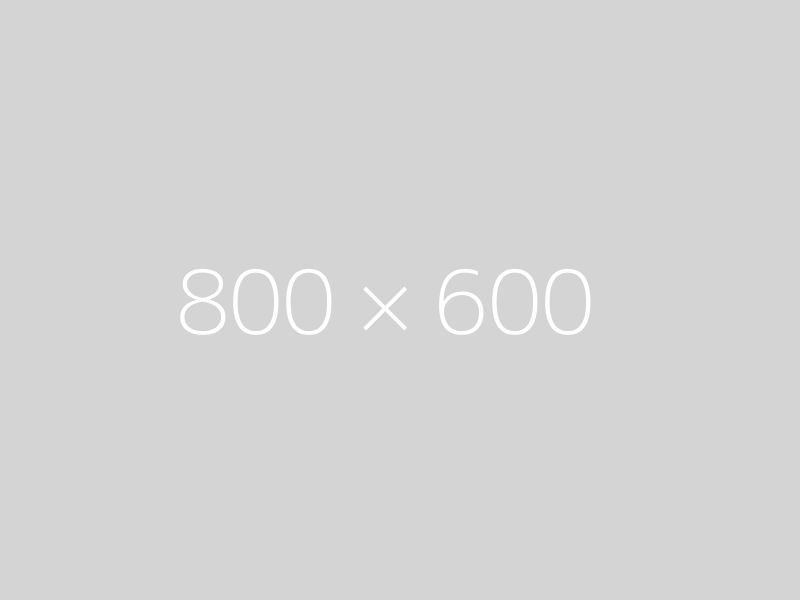
\includegraphics[width=\textwidth]{figures/placeholder.png}
    \caption[An example Figure 1.]{\textbf{An example Figure 1.} An example 800x600 figure, that should be displayed in a new page. If you don't like it, then check this web page for more information on the figure positioning: \href{https://www.overleaf.com/learn/latex/Positioning_of_Figures}{https://www.overleaf.com/learn/latex/Positioning\_of\_Figures}}
    \label{figlabel1}
\end{figure}

Aenean mollis viverra elit, a ullamcorper tortor mollis et. Mauris ultricies turpis nec lacinia pulvinar. Ut mollis tortor dapibus, dapibus nibh vel, condimentum mauris. Aenean neque velit, dignissim at nulla a, pharetra mattis sapien. Pellentesque in scelerisque justo. Nullam mattis nisi eget elit elementum gravida. Etiam posuere sollicitudin libero ac imperdiet.

\subsection{This is a subsection}
Etiam aliquam libero ante. Cras sagittis dolor lectus, id malesuada mauris rhoncus ut. Etiam at nisl ut ligula lacinia mollis id nec quam. In finibus neque id ex viverra, quis commodo augue aliquet. Etiam ultricies feugiat congue. Lorem ipsum dolor sit amet, consectetur adipiscing elit. Cras hendrerit maximus dolor ut auctor. Mauris porttitor gravida eros, id porta odio fermentum id. Nullam erat ligula, interdum sit amet justo nec, auctor sagittis augue. Phasellus accumsan rhoncus consequat.

\subsubsection{This is a subsubsection}
Aenean ullamcorper suscipit laoreet. Vestibulum fermentum quam urna, eu venenatis dui venenatis in. Aenean id purus efficitur, venenatis mi non, iaculis sapien. Vestibulum ante ipsum primis in faucibus orci luctus et ultrices posuere cubilia Curae; Donec a sem non arcu luctus egestas aliquam vel magna. Ut congue lorem eu ante congue accumsan. Mauris eget magna vulputate, euismod odio in, aliquam quam. Phasellus purus ante, congue id laoreet quis, consequat a mauris. Quisque aliquet, nunc vel vestibulum faucibus, diam nibh maximus massa, eu finibus ligula eros eu ipsum. Integer posuere mauris non enim convallis, in dictum ipsum porttitor. Proin dictum semper lorem ut semper. Aenean tempus commodo leo, vel hendrerit est dapibus nec. Sed feugiat, augue quis mollis ultrices, ex elit imperdiet purus, quis venenatis arcu magna vitae orci. Duis malesuada turpis mi, sit amet convallis urna mollis ac. Pellentesque habitant morbi tristique senectus et netus et malesuada fames ac turpis egestas. Integer vel nisl urna.

\begin{equation} \label{eq1}
\begin{aligned}
    S_i &= \sum^5_{a=1}\frac{F_i-1}{D_i}\times\frac{R_{i-4+G+a}-1}{D_{i-4+G+a}}\times(F_i+R_{i-4+G+a}-2) \\
    &+ \sum^5_{a=1}\frac{R_{i-1+G}-1}{D_{i-1+G}}\times\frac{F_{i-3+a}-1}{D_{i-3+a}}\times(R_{i-1+G}+F_{i-3+a}-2)
\end{aligned}
\end{equation}
where:
\begin{conditions}
\quad F_i & Number of forward sequence reads starting at position i \\
\quad R_i & Number of reverse sequence reads starting at position i \\
\quad D_i & Sequencing depth at position i \\
\quad G   & Size of sticky end overhang (positive/negative value for 5'/3' overhang)
\end{conditions}

Vivamus felis mi, pellentesque sit amet diam ac, accumsan viverra lectus. Curabitur vulputate nisl ac mauris dignissim pharetra. In nec dui nec diam ultrices viverra. In laoreet nisl nec lobortis blandit. Aliquam efficitur odio at porttitor semper. Mauris metus diam, malesuada id faucibus a, convallis eu turpis. Quisque sit amet consequat neque. Suspendisse porttitor ac odio et interdum. Nunc efficitur quis mi ultricies volutpat. Pellentesque posuere eros vitae ex lacinia, in lobortis tellus ullamcorper. Aliquam risus nunc, mattis dignissim pharetra non, cursus eu leo. Vestibulum tincidunt enim a sapien fringilla, at ultricies sem hendrerit. Pellentesque imperdiet, mi a scelerisque accumsan, dui ex molestie nulla, a consectetur elit ex ac neque. Maecenas pellentesque metus vitae porttitor cursus. Sed non dolor consectetur magna commodo commodo.

Suspendisse interdum tincidunt odio, a rutrum lorem semper in. Sed iaculis odio magna, in mattis tellus tempus ut. Vivamus ut ornare nulla, sed semper ex. Maecenas tempor interdum quam. Mauris ac turpis efficitur, faucibus metus et, ultricies tellus. Vivamus tincidunt purus elit, nec cursus ante accumsan vel. Vestibulum faucibus diam in sollicitudin viverra. Sed fermentum eget elit ac maximus. Phasellus tempor rutrum lacinia. Integer elementum diam erat. Suspendisse ac mi arcu. Vestibulum dui ante, scelerisque a sapien ut, iaculis fermentum turpis. Donec ac faucibus metus, quis consectetur felis. Sed ornare diam vel sapien mattis efficitur. Aliquam eget urna massa. Integer massa nisl, tristique eu congue ut, ullamcorper in tortor.

Morbi ullamcorper nunc et urna euismod ullamcorper. Proin tincidunt pretium velit, sollicitudin fringilla dolor imperdiet at. Aliquam lobortis tempus velit, ut ultrices leo finibus in. Integer quis diam et risus lacinia sodales. Pellentesque nisl purus, placerat eu turpis id, fringilla consequat neque. Sed eu nisi lacus. Cras tempus tempor elit. Proin dapibus tempor lorem at venenatis. Donec eu vestibulum augue, at elementum nisl.

Praesent cursus odio ac efficitur mollis. Vestibulum ante ipsum primis in faucibus orci luctus et ultrices posuere cubilia Curae; Vestibulum venenatis eget est scelerisque vulputate. Maecenas commodo, mi eu dignissim rutrum, orci lorem mollis eros, eget auctor augue arcu congue metus. Nulla feugiat orci ac ex ultrices accumsan. Duis faucibus sit amet enim vel pulvinar. Mauris lacinia varius elementum. Aenean dapibus felis sit amet orci fringilla, sit amet hendrerit quam scelerisque.

\section{Yet another Section}
Lorem ipsum dolor sit amet, consectetur adipiscing elit. Integer ut leo luctus, placerat sapien ultrices, porttitor leo. In a ligula elementum, bibendum sapien quis, mattis mi. Proin dapibus pulvinar magna, id vulputate tortor auctor quis. Mauris in felis sed enim tristique pretium a eget massa. Sed pharetra mattis dignissim. Pellentesque vel nibh elit. Maecenas erat nisl, lacinia et massa vitae, tincidunt venenatis leo. Nam sollicitudin enim quam, in vehicula lacus rhoncus eu. Mauris convallis leo et lectus efficitur, ac bibendum erat bibendum. Donec velit nulla, bibendum eu hendrerit in, sollicitudin ut tellus.

Vestibulum lobortis enim vitae ante luctus, egestas pulvinar ante gravida. Vivamus elementum elit purus, nec feugiat augue ultricies tincidunt. Aenean efficitur dui quam, at gravida risus semper quis. Quisque finibus ut mi vitae tincidunt. Aliquam erat volutpat. Sed ac odio eget nisl vulputate tempor id sed lorem. Nulla sit amet lorem at lacus rhoncus volutpat. Fusce consectetur magna sed auctor porttitor. Proin dignissim elit non condimentum interdum. Nulla laoreet fringilla sapien sed eleifend. Phasellus eget lectus in ipsum tincidunt mattis. Vivamus mauris lacus, varius non sem ultrices, varius consequat arcu. Quisque ut dolor eget massa pharetra blandit sit amet ut turpis.

Phasellus ullamcorper facilisis lobortis. Ut quis ligula venenatis, rhoncus urna vitae, lobortis augue. Nam faucibus justo sem, quis mattis nulla sodales luctus. Donec fermentum vulputate sapien, vitae scelerisque tellus pharetra et. Curabitur dignissim hendrerit sollicitudin. Vivamus in lacus urna. Nam mollis felis vitae purus interdum, id bibendum magna aliquam. In hac habitasse platea dictumst. Sed maximus ullamcorper lorem, eleifend venenatis enim varius in.

Praesent fermentum metus neque, vitae pretium lectus tincidunt non. Curabitur mollis tortor felis, eu molestie libero faucibus eu. Nullam vitae mi orci. Praesent eget nisi at tortor lacinia rhoncus eget eu lorem. Vivamus consectetur sem ac mi ultricies, non tempus enim scelerisque. Suspendisse potenti. Vivamus eu convallis metus. Maecenas quis pharetra nisl, vel feugiat ipsum. Fusce elementum nibh vitae sollicitudin iaculis. Mauris consectetur augue a dictum pellentesque. Suspendisse blandit mattis luctus.

Suspendisse laoreet mi ac feugiat placerat. In ut diam in erat cursus aliquet nec eu felis. Praesent ut dolor quis quam consectetur elementum. Etiam nec volutpat leo, a semper nibh. Curabitur semper condimentum metus sed feugiat. In non finibus nibh. Nam laoreet odio id lacus fermentum blandit. Maecenas feugiat quis lorem eget ullamcorper. Vivamus volutpat convallis mi at tempor.

\section{The Final Section}
Lorem ipsum dolor sit amet, consectetur adipiscing elit. Integer ut leo luctus, placerat sapien ultrices, porttitor leo. In a ligula elementum, bibendum sapien quis, mattis mi. Proin dapibus pulvinar magna, id vulputate tortor auctor quis. Mauris in felis sed enim tristique pretium a eget massa. Sed pharetra mattis dignissim. Pellentesque vel nibh elit. Maecenas erat nisl, lacinia et massa vitae, tincidunt venenatis leo. Nam sollicitudin enim quam, in vehicula lacus rhoncus eu. Mauris convallis leo et lectus efficitur, ac bibendum erat bibendum. Donec velit nulla, bibendum eu hendrerit in, sollicitudin ut tellus.

Vestibulum lobortis enim vitae ante luctus, egestas pulvinar ante gravida. Vivamus elementum elit purus, nec feugiat augue ultricies tincidunt. Aenean efficitur dui quam, at gravida risus semper quis. Quisque finibus ut mi vitae tincidunt. Aliquam erat volutpat. Sed ac odio eget nisl vulputate tempor id sed lorem. Nulla sit amet lorem at lacus rhoncus volutpat. Fusce consectetur magna sed auctor porttitor. Proin dignissim elit non condimentum interdum. Nulla laoreet fringilla sapien sed eleifend. Phasellus eget lectus in ipsum tincidunt mattis. Vivamus mauris lacus, varius non sem ultrices, varius consequat arcu. Quisque ut dolor eget massa pharetra blandit sit amet ut turpis.

Phasellus ullamcorper facilisis lobortis. Ut quis ligula venenatis, rhoncus urna vitae, lobortis augue. Nam faucibus justo sem, quis mattis nulla sodales luctus. Donec fermentum vulputate sapien, vitae scelerisque tellus pharetra et. Curabitur dignissim hendrerit sollicitudin. Vivamus in lacus urna. Nam mollis felis vitae purus interdum, id bibendum magna aliquam. In hac habitasse platea dictumst. Sed maximus ullamcorper lorem, eleifend venenatis enim varius in.
\chapter{The Second Chapter}
\section{The First Section}
Lorem ipsum dolor sit amet, consectetur adipiscing elit. Sed aliquam elit at massa sodales, eu imperdiet ligula feugiat. Quisque nec eros sodales, pretium est sodales, iaculis lorem. Suspendisse in semper diam, nec mollis urna. Aliquam gravida lobortis ligula. Fusce pulvinar mi ipsum. Ut nibh turpis, auctor vitae interdum sit amet, fermentum non turpis. Praesent vel risus commodo, dapibus enim ac, maximus neque. Duis convallis, massa et cursus dapibus, leo erat mattis neque, ac interdum quam tortor sit amet justo. Morbi ac dui interdum, posuere risus a, pulvinar mi. Maecenas faucibus consequat suscipit. Maecenas lacinia sit amet tellus sed molestie. Suspendisse bibendum commodo dolor, vitae pulvinar lorem condimentum vitae. Sed molestie condimentum pharetra. Etiam viverra lobortis mi, a vehicula sem convallis id. Etiam gravida arcu et tellus scelerisque ultricies. Cras sed porta ipsum, sed consectetur lorem.

\begin{figure}[p]
    \centering
    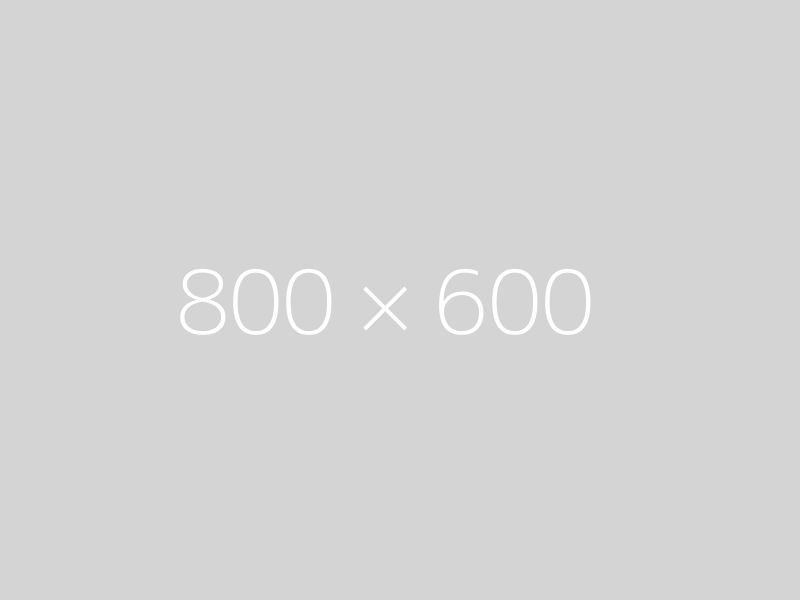
\includegraphics[width=\textwidth]{figures/placeholder.png}
    \caption[An example Figure 2.]{\textbf{An example Figure 2.} An example 800x600 figure, that should be displayed in a new page.}
    \label{figlabel2}
\end{figure}

Aenean mollis viverra elit, a ullamcorper tortor mollis et. Mauris ultricies turpis nec lacinia pulvinar. Ut mollis tortor dapibus, dapibus nibh vel, condimentum mauris. Aenean neque velit, dignissim at nulla a, pharetra mattis sapien. Pellentesque in scelerisque justo. Nullam mattis nisi eget elit elementum gravida. Etiam posuere sollicitudin libero ac imperdiet.

\subsection{This is a subsection}
Etiam aliquam libero ante. Cras sagittis dolor lectus, id malesuada mauris rhoncus ut. Etiam at nisl ut ligula lacinia mollis id nec quam. In finibus neque id ex viverra, quis commodo augue aliquet. Etiam ultricies feugiat congue. Lorem ipsum dolor sit amet, consectetur adipiscing elit. Cras hendrerit maximus dolor ut auctor. Mauris porttitor gravida eros, id porta odio fermentum id. Nullam erat ligula, interdum sit amet justo nec, auctor sagittis augue. Phasellus accumsan rhoncus consequat.

\subsubsection{This is a subsubsection}
Aenean ullamcorper suscipit laoreet. Vestibulum fermentum quam urna, eu venenatis dui venenatis in. Aenean id purus efficitur, venenatis mi non, iaculis sapien. Vestibulum ante ipsum primis in faucibus orci luctus et ultrices posuere cubilia Curae; Donec a sem non arcu luctus egestas aliquam vel magna. Ut congue lorem eu ante congue accumsan. Mauris eget magna vulputate, euismod odio in, aliquam quam. Phasellus purus ante, congue id laoreet quis, consequat a mauris. Quisque aliquet, nunc vel vestibulum faucibus, diam nibh maximus massa, eu finibus ligula eros eu ipsum. Integer posuere mauris non enim convallis, in dictum ipsum porttitor. Proin dictum semper lorem ut semper. Aenean tempus commodo leo, vel hendrerit est dapibus nec. Sed feugiat, augue quis mollis ultrices, ex elit imperdiet purus, quis venenatis arcu magna vitae orci. Duis malesuada turpis mi, sit amet convallis urna mollis ac. Pellentesque habitant morbi tristique senectus et netus et malesuada fames ac turpis egestas. Integer vel nisl urna.

\subsection{Yet another subsection}
Vivamus felis mi, pellentesque sit amet diam ac, accumsan viverra lectus. Curabitur vulputate nisl ac mauris dignissim pharetra. In nec dui nec diam ultrices viverra. In laoreet nisl nec lobortis blandit. Aliquam efficitur odio at porttitor semper. Mauris metus diam, malesuada id faucibus a, convallis eu turpis. Quisque sit amet consequat neque. Suspendisse porttitor ac odio et interdum. Nunc efficitur quis mi ultricies volutpat. Pellentesque posuere eros vitae ex lacinia, in lobortis tellus ullamcorper. Aliquam risus nunc, mattis dignissim pharetra non, cursus eu leo. Vestibulum tincidunt enim a sapien fringilla, at ultricies sem hendrerit. Pellentesque imperdiet, mi a scelerisque accumsan, dui ex molestie nulla, a consectetur elit ex ac neque. Maecenas pellentesque metus vitae porttitor cursus. Sed non dolor consectetur magna commodo commodo.

Suspendisse interdum tincidunt odio, a rutrum lorem semper in. Sed iaculis odio magna, in mattis tellus tempus ut. Vivamus ut ornare nulla, sed semper ex. Maecenas tempor interdum quam. Mauris ac turpis efficitur, faucibus metus et, ultricies tellus. Vivamus tincidunt purus elit, nec cursus ante accumsan vel. Vestibulum faucibus diam in sollicitudin viverra. Sed fermentum eget elit ac maximus. Phasellus tempor rutrum lacinia. Integer elementum diam erat. Suspendisse ac mi arcu. Vestibulum dui ante, scelerisque a sapien ut, iaculis fermentum turpis. Donec ac faucibus metus, quis consectetur felis. Sed ornare diam vel sapien mattis efficitur. Aliquam eget urna massa. Integer massa nisl, tristique eu congue ut, ullamcorper in tortor.

Morbi ullamcorper nunc et urna euismod ullamcorper. Proin tincidunt pretium velit, sollicitudin fringilla dolor imperdiet at. Aliquam lobortis tempus velit, ut ultrices leo finibus in. Integer quis diam et risus lacinia sodales. Pellentesque nisl purus, placerat eu turpis id, fringilla consequat neque. Sed eu nisi lacus. Cras tempus tempor elit. Proin dapibus tempor lorem at venenatis. Donec eu vestibulum augue, at elementum nisl.

Praesent cursus odio ac efficitur mollis. Vestibulum ante ipsum primis in faucibus orci luctus et ultrices posuere cubilia Curae; Vestibulum venenatis eget est scelerisque vulputate. Maecenas commodo, mi eu dignissim rutrum, orci lorem mollis eros, eget auctor augue arcu congue metus. Nulla feugiat orci ac ex ultrices accumsan. Duis faucibus sit amet enim vel pulvinar. Mauris lacinia varius elementum. Aenean dapibus felis sit amet orci fringilla, sit amet hendrerit quam scelerisque.

\section{Another Section}
Lorem ipsum dolor sit amet, consectetur adipiscing elit. Integer ut leo luctus, placerat sapien ultrices, porttitor leo. In a ligula elementum, bibendum sapien quis, mattis mi. Proin dapibus pulvinar magna, id vulputate tortor auctor quis. Mauris in felis sed enim tristique pretium a eget massa. Sed pharetra mattis dignissim. Pellentesque vel nibh elit. Maecenas erat nisl, lacinia et massa vitae, tincidunt venenatis leo. Nam sollicitudin enim quam, in vehicula lacus rhoncus eu. Mauris convallis leo et lectus efficitur, ac bibendum erat bibendum. Donec velit nulla, bibendum eu hendrerit in, sollicitudin ut tellus.

Vestibulum lobortis enim vitae ante luctus, egestas pulvinar ante gravida. Vivamus elementum elit purus, nec feugiat augue ultricies tincidunt. Aenean efficitur dui quam, at gravida risus semper quis. Quisque finibus ut mi vitae tincidunt. Aliquam erat volutpat. Sed ac odio eget nisl vulputate tempor id sed lorem. Nulla sit amet lorem at lacus rhoncus volutpat. Fusce consectetur magna sed auctor porttitor. Proin dignissim elit non condimentum interdum. Nulla laoreet fringilla sapien sed eleifend. Phasellus eget lectus in ipsum tincidunt mattis. Vivamus mauris lacus, varius non sem ultrices, varius consequat arcu. Quisque ut dolor eget massa pharetra blandit sit amet ut turpis.

\begin{table}[t]
\centering
\begin{tabular}{llr}
\hline
\multicolumn{2}{c}{Item} &           \\ \cline{1-2}
Animal     & Description & Price (\$) \\ \hline
Gnat       & per gram    & 13.65     \\
           & each        & 0.01      \\
Gnu        & stuffed     & 92.50     \\
Emu        & stuffed     & 33.33     \\
Armadillo  & frozen      & 8.99      \\ \hline
\end{tabular}
\caption[An example table.]{\textbf{An example table.} Check this awesome website for creating \LaTeX{} tables! \href{https://www.tablesgenerator.com/}{https://www.tablesgenerator.com/}}
\label{tab:my-table}
\end{table}

Phasellus ullamcorper facilisis lobortis. Ut quis ligula venenatis, rhoncus urna vitae, lobortis augue. Nam faucibus justo sem, quis mattis nulla sodales luctus. Donec fermentum vulputate sapien, vitae scelerisque tellus pharetra et. Curabitur dignissim hendrerit sollicitudin. Vivamus in lacus urna. Nam mollis felis vitae purus interdum, id bibendum magna aliquam. In hac habitasse platea dictumst. Sed maximus ullamcorper lorem, eleifend venenatis enim varius in.

Praesent fermentum metus neque, vitae pretium lectus tincidunt non. Curabitur mollis tortor felis, eu molestie libero faucibus eu. Nullam vitae mi orci. Praesent eget nisi at tortor lacinia rhoncus eget eu lorem. Vivamus consectetur sem ac mi ultricies, non tempus enim scelerisque. Suspendisse potenti. Vivamus eu convallis metus. Maecenas quis pharetra nisl, vel feugiat ipsum. Fusce elementum nibh vitae sollicitudin iaculis. Mauris consectetur augue a dictum pellentesque. Suspendisse blandit mattis luctus.

Suspendisse laoreet mi ac feugiat placerat. In ut diam in erat cursus aliquet nec eu felis. Praesent ut dolor quis quam consectetur elementum. Etiam nec volutpat leo, a semper nibh. Curabitur semper condimentum metus sed feugiat. In non finibus nibh. Nam laoreet odio id lacus fermentum blandit. Maecenas feugiat quis lorem eget ullamcorper. Vivamus volutpat convallis mi at tempor.

\section{The Final Section}
Lorem ipsum dolor sit amet, consectetur adipiscing elit. Integer ut leo luctus, placerat sapien ultrices, porttitor leo. In a ligula elementum, bibendum sapien quis, mattis mi. Proin dapibus pulvinar magna, id vulputate tortor auctor quis. Mauris in felis sed enim tristique pretium a eget massa. Sed pharetra mattis dignissim. Pellentesque vel nibh elit. Maecenas erat nisl, lacinia et massa vitae, tincidunt venenatis leo. Nam sollicitudin enim quam, in vehicula lacus rhoncus eu. Mauris convallis leo et lectus efficitur, ac bibendum erat bibendum. Donec velit nulla, bibendum eu hendrerit in, sollicitudin ut tellus.

Vestibulum lobortis enim vitae ante luctus, egestas pulvinar ante gravida. Vivamus elementum elit purus, nec feugiat augue ultricies tincidunt. Aenean efficitur dui quam, at gravida risus semper quis. Quisque finibus ut mi vitae tincidunt. Aliquam erat volutpat. Sed ac odio eget nisl vulputate tempor id sed lorem. Nulla sit amet lorem at lacus rhoncus volutpat. Fusce consectetur magna sed auctor porttitor. Proin dignissim elit non condimentum interdum. Nulla laoreet fringilla sapien sed eleifend. Phasellus eget lectus in ipsum tincidunt mattis. Vivamus mauris lacus, varius non sem ultrices, varius consequat arcu. Quisque ut dolor eget massa pharetra blandit sit amet ut turpis.

Phasellus ullamcorper facilisis lobortis. Ut quis ligula venenatis, rhoncus urna vitae, lobortis augue. Nam faucibus justo sem, quis mattis nulla sodales luctus. Donec fermentum vulputate sapien, vitae scelerisque tellus pharetra et. Curabitur dignissim hendrerit sollicitudin. Vivamus in lacus urna. Nam mollis felis vitae purus interdum, id bibendum magna aliquam. In hac habitasse platea dictumst. Sed maximus ullamcorper lorem, eleifend venenatis enim varius in.

Praesent fermentum metus neque, vitae pretium lectus tincidunt non. Curabitur mollis tortor felis, eu molestie libero faucibus eu. Nullam vitae mi orci. Praesent eget nisi at tortor lacinia rhoncus eget eu lorem. Vivamus consectetur sem ac mi ultricies, non tempus enim scelerisque. Suspendisse potenti. Vivamus eu convallis metus. Maecenas quis pharetra nisl, vel feugiat ipsum. Fusce elementum nibh vitae sollicitudin iaculis. Mauris consectetur augue a dictum pellentesque. Suspendisse blandit mattis luctus.

Fusce viverra enim enim, vitae ornare lacus imperdiet sit amet. Maecenas eu finibus urna. Suspendisse ornare dolor vitae volutpat porttitor. Morbi nibh est, tincidunt ac rhoncus at, tristique eu dui. Class aptent taciti sociosqu ad litora torquent per conubia nostra, per inceptos himenaeos. Nunc cursus magna sit amet ex iaculis, vel auctor nisl cursus. Fusce eleifend mattis ante, vel varius urna hendrerit ut. Nunc condimentum nisl eget augue accumsan dignissim. Nunc gravida convallis risus at mattis. Donec viverra egestas eros, facilisis ultricies augue cursus vel. Cras dapibus dolor eu purus pulvinar pharetra. Nunc iaculis, risus sed accumsan suscipit, leo nisl lobortis metus, ut malesuada dui magna id ante. Suspendisse vel neque in erat interdum consequat. Ut hendrerit, augue a tristique finibus, urna nibh pretium leo, sed vestibulum dui lacus in neque.

Aenean molestie felis sit amet nulla consequat viverra. Etiam tempus auctor turpis nec venenatis. Vestibulum eu nisi odio. Quisque lectus ante, placerat a eros a, venenatis bibendum nunc. Aenean efficitur maximus tortor, in congue dolor consectetur id. Integer placerat tempor metus, a ornare ipsum vestibulum nec. Morbi lobortis dictum viverra. Etiam id pellentesque neque, vel auctor sem. Nulla posuere sagittis nulla, quis hendrerit nulla suscipit id. Maecenas risus risus, congue in condimentum nec, ullamcorper in lorem. Donec lectus massa, tempor fringilla sollicitudin non, dapibus sed risus.

Etiam ut lorem eget massa convallis ornare vitae a orci. Nunc placerat libero id nisl tempus, vel euismod sem imperdiet. Suspendisse mollis risus sed mauris imperdiet tristique. Proin tortor ex, pharetra at nisl a, pellentesque aliquam enim. Pellentesque eleifend purus id lorem euismod sodales. Vestibulum ac massa tincidunt, semper erat sed, faucibus arcu. Nunc condimentum ex pulvinar leo interdum convallis. Aliquam ac posuere ligula. Vivamus dui nisl, efficitur varius libero vel, pharetra porta ante. Orci varius natoque penatibus et magnis dis parturient montes, nascetur ridiculus mus. Etiam et ipsum eget lacus tincidunt pellentesque. Orci varius natoque penatibus et magnis dis parturient montes, nascetur ridiculus mus.

Pellentesque a ultrices ex. Curabitur commodo a diam ut luctus. Nulla in augue sodales, suscipit lacus vel, vehicula ante. Suspendisse fermentum mattis risus eget volutpat. Ut justo tellus, tempor a ligula hendrerit, ornare pellentesque nisi. Etiam elementum mollis sagittis. Nullam dignissim eget eros vitae scelerisque. Integer vitae tempus felis, vitae tincidunt enim. Curabitur mauris velit, scelerisque in tristique in, efficitur in augue. Sed quis diam et mauris efficitur lacinia. Duis ultricies dolor in consequat dapibus. Curabitur tristique neque a cursus vestibulum. Sed viverra consectetur orci, quis posuere tortor euismod non. Fusce eget molestie nulla, a lacinia dui. Lorem ipsum dolor sit amet, consectetur adipiscing elit. Pellentesque eget varius nisi, id congue elit.
\chapter{The Third Chapter}
\section{The First Section}
Lorem ipsum dolor sit amet, consectetur adipiscing elit. Sed aliquam elit at massa sodales, eu imperdiet ligula feugiat. Quisque nec eros sodales, pretium est sodales, iaculis lorem. Suspendisse in semper diam, nec mollis urna. Aliquam gravida lobortis ligula. Fusce pulvinar mi ipsum. Ut nibh turpis, auctor vitae interdum sit amet, fermentum non turpis. Praesent vel risus commodo, dapibus enim ac, maximus neque. Duis convallis, massa et cursus dapibus, leo erat mattis neque, ac interdum quam tortor sit amet justo. Morbi ac dui interdum, posuere risus a, pulvinar mi. Maecenas faucibus consequat suscipit. Maecenas lacinia sit amet tellus sed molestie. Suspendisse bibendum commodo dolor, vitae pulvinar lorem condimentum vitae. Sed molestie condimentum pharetra. Etiam viverra lobortis mi, a vehicula sem convallis id. Etiam gravida arcu et tellus scelerisque ultricies. Cras sed porta ipsum, sed consectetur lorem.

\begin{figure}[p]
    \centering
    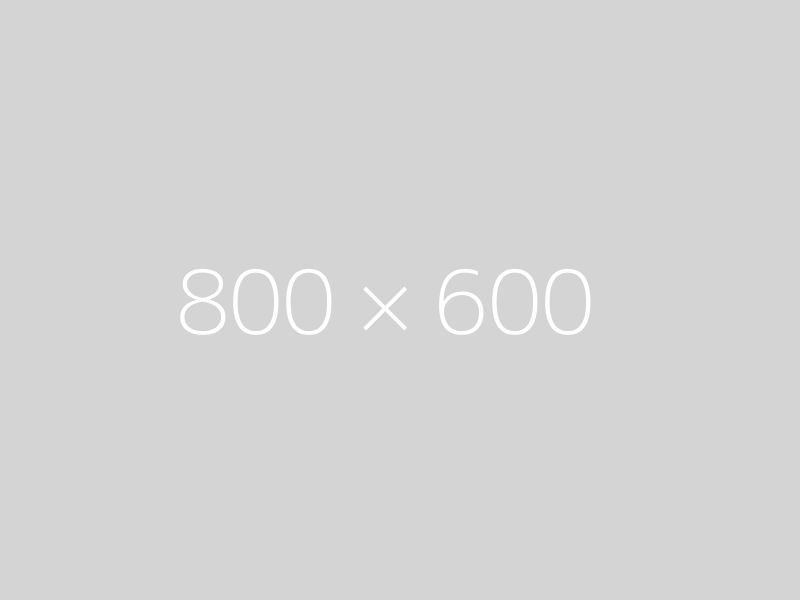
\includegraphics[width=\textwidth]{figures/placeholder.png}
    \caption[An example Figure 3.]{\textbf{An example Figure 3.} An example 800x600 figure, that should be displayed in a new page.}
    \label{figlabel3}
\end{figure}

Aenean mollis viverra elit, a ullamcorper tortor mollis et. Mauris ultricies turpis nec lacinia pulvinar. Ut mollis tortor dapibus, dapibus nibh vel, condimentum mauris. Aenean neque velit, dignissim at nulla a, pharetra mattis sapien. Pellentesque in scelerisque justo. Nullam mattis nisi eget elit elementum gravida. Etiam posuere sollicitudin libero ac imperdiet.

\section{Another Section}
Lorem ipsum dolor sit amet, consectetur adipiscing elit. Integer ut leo luctus, placerat sapien ultrices, porttitor leo. In a ligula elementum, bibendum sapien quis, mattis mi. Proin dapibus pulvinar magna, id vulputate tortor auctor quis. Mauris in felis sed enim tristique pretium a eget massa. Sed pharetra mattis dignissim. Pellentesque vel nibh elit. Maecenas erat nisl, lacinia et massa vitae, tincidunt venenatis leo. Nam sollicitudin enim quam, in vehicula lacus rhoncus eu. Mauris convallis leo et lectus efficitur, ac bibendum erat bibendum. Donec velit nulla, bibendum eu hendrerit in, sollicitudin ut tellus.

Vestibulum lobortis enim vitae ante luctus, egestas pulvinar ante gravida. Vivamus elementum elit purus, nec feugiat augue ultricies tincidunt. Aenean efficitur dui quam, at gravida risus semper quis. Quisque finibus ut mi vitae tincidunt. Aliquam erat volutpat. Sed ac odio eget nisl vulputate tempor id sed lorem. Nulla sit amet lorem at lacus rhoncus volutpat. Fusce consectetur magna sed auctor porttitor. Proin dignissim elit non condimentum interdum. Nulla laoreet fringilla sapien sed eleifend. Phasellus eget lectus in ipsum tincidunt mattis. Vivamus mauris lacus, varius non sem ultrices, varius consequat arcu. Quisque ut dolor eget massa pharetra blandit sit amet ut turpis.

Phasellus ullamcorper facilisis lobortis. Ut quis ligula venenatis, rhoncus urna vitae, lobortis augue. Nam faucibus justo sem, quis mattis nulla sodales luctus. Donec fermentum vulputate sapien, vitae scelerisque tellus pharetra et. Curabitur dignissim hendrerit sollicitudin. Vivamus in lacus urna. Nam mollis felis vitae purus interdum, id bibendum magna aliquam. In hac habitasse platea dictumst. Sed maximus ullamcorper lorem, eleifend venenatis enim varius in.

Praesent fermentum metus neque, vitae pretium lectus tincidunt non. Curabitur mollis tortor felis, eu molestie libero faucibus eu. Nullam vitae mi orci. Praesent eget nisi at tortor lacinia rhoncus eget eu lorem. Vivamus consectetur sem ac mi ultricies, non tempus enim scelerisque. Suspendisse potenti. Vivamus eu convallis metus. Maecenas quis pharetra nisl, vel feugiat ipsum. Fusce elementum nibh vitae sollicitudin iaculis. Mauris consectetur augue a dictum pellentesque. Suspendisse blandit mattis luctus.

Suspendisse laoreet mi ac feugiat placerat. In ut diam in erat cursus aliquet nec eu felis. Praesent ut dolor quis quam consectetur elementum. Etiam nec volutpat leo, a semper nibh. Curabitur semper condimentum metus sed feugiat. In non finibus nibh. Nam laoreet odio id lacus fermentum blandit. Maecenas feugiat quis lorem eget ullamcorper. Vivamus volutpat convallis mi at tempor.

\section{The Final Section}
Lorem ipsum dolor sit amet, consectetur adipiscing elit. Integer ut leo luctus, placerat sapien ultrices, porttitor leo. In a ligula elementum, bibendum sapien quis, mattis mi. Proin dapibus pulvinar magna, id vulputate tortor auctor quis. Mauris in felis sed enim tristique pretium a eget massa. Sed pharetra mattis dignissim. Pellentesque vel nibh elit. Maecenas erat nisl, lacinia et massa vitae, tincidunt venenatis leo. Nam sollicitudin enim quam, in vehicula lacus rhoncus eu. Mauris convallis leo et lectus efficitur, ac bibendum erat bibendum. Donec velit nulla, bibendum eu hendrerit in, sollicitudin ut tellus.

Vestibulum lobortis enim vitae ante luctus, egestas pulvinar ante gravida. Vivamus elementum elit purus, nec feugiat augue ultricies tincidunt. Aenean efficitur dui quam, at gravida risus semper quis. Quisque finibus ut mi vitae tincidunt. Aliquam erat volutpat. Sed ac odio eget nisl vulputate tempor id sed lorem. Nulla sit amet lorem at lacus rhoncus volutpat. Fusce consectetur magna sed auctor porttitor. Proin dignissim elit non condimentum interdum. Nulla laoreet fringilla sapien sed eleifend. Phasellus eget lectus in ipsum tincidunt mattis. Vivamus mauris lacus, varius non sem ultrices, varius consequat arcu. Quisque ut dolor eget massa pharetra blandit sit amet ut turpis.

Phasellus ullamcorper facilisis lobortis. Ut quis ligula venenatis, rhoncus urna vitae, lobortis augue. Nam faucibus justo sem, quis mattis nulla sodales luctus. Donec fermentum vulputate sapien, vitae scelerisque tellus pharetra et. Curabitur dignissim hendrerit sollicitudin. Vivamus in lacus urna. Nam mollis felis vitae purus interdum, id bibendum magna aliquam. In hac habitasse platea dictumst. Sed maximus ullamcorper lorem, eleifend venenatis enim varius in.

Praesent fermentum metus neque, vitae pretium lectus tincidunt non. Curabitur mollis tortor felis, eu molestie libero faucibus eu. Nullam vitae mi orci. Praesent eget nisi at tortor lacinia rhoncus eget eu lorem. Vivamus consectetur sem ac mi ultricies, non tempus enim scelerisque. Suspendisse potenti. Vivamus eu convallis metus. Maecenas quis pharetra nisl, vel feugiat ipsum. Fusce elementum nibh vitae sollicitudin iaculis. Mauris consectetur augue a dictum pellentesque. Suspendisse blandit mattis luctus.

Suspendisse laoreet mi ac feugiat placerat. In ut diam in erat cursus aliquet nec eu felis. Praesent ut dolor quis quam consectetur elementum. Etiam nec volutpat leo, a semper nibh. Curabitur semper condimentum metus sed feugiat. In non finibus nibh. Nam laoreet odio id lacus fermentum blandit. Maecenas feugiat quis lorem eget ullamcorper. Vivamus volutpat convallis mi at tempor.

Cras tempor, leo sed rutrum molestie, metus leo blandit sem, sed ultrices quam dui eget nisl. Nulla sit amet velit ut eros ornare venenatis. Vivamus gravida finibus neque id pharetra. Mauris ex tortor, aliquam quis tempor sed, mollis at felis. Nulla facilisi. Vestibulum imperdiet nibh et sollicitudin bibendum. Interdum et malesuada fames ac ante ipsum primis in faucibus. Aenean tristique turpis a lorem auctor ornare. Donec aliquam ex in diam imperdiet, a semper mi tincidunt. Aenean vehicula urna lacus, suscipit gravida nunc fringilla nec. Pellentesque eget ex sit amet erat ornare pulvinar at eget orci. Nam sed ante et leo placerat viverra non at urna. Vivamus pretium ut enim sit amet aliquam. Nullam iaculis velit vel odio congue, non tempus lectus aliquet. Sed pharetra porttitor orci.

Vestibulum in tincidunt elit. Ut rutrum ante a pharetra interdum. Etiam eu turpis a purus cursus viverra. Nunc pretium tellus vehicula orci vestibulum, aliquam rhoncus ligula consectetur. Curabitur laoreet, lorem vitae pulvinar posuere, dolor risus blandit neque, id maximus ipsum nisi vitae magna. Sed in diam nec orci facilisis congue in a dolor. Aliquam quis ex sem. Maecenas pharetra magna elit, ut volutpat diam mattis pulvinar. Morbi euismod congue dui id porttitor. Duis vestibulum diam vitae tortor egestas pulvinar. Fusce vulputate vitae nulla id volutpat. Donec metus diam, varius eget pulvinar id, maximus sit amet lacus.

Pellentesque commodo lorem sit amet ligula imperdiet, vitae convallis velit ullamcorper. Etiam euismod ex id nisi malesuada congue. Pellentesque vel viverra mauris. Integer rhoncus bibendum dolor, in lobortis erat aliquam nec. Nullam non quam enim. Ut purus massa, finibus nec justo bibendum, maximus pretium justo. Nullam malesuada eros ut velit facilisis, sit amet ultrices odio porta. Phasellus imperdiet lorem velit, quis fermentum lorem porta et. Aenean eleifend consectetur arcu, pellentesque mollis tortor tempus quis. Nulla volutpat viverra ullamcorper. Nunc vehicula mauris eget orci efficitur rhoncus. Aenean dapibus varius convallis. Etiam facilisis eleifend malesuada. In magna ante, ullamcorper ut fringilla ac, interdum vel tellus.

Duis laoreet dapibus lectus, sed interdum ligula egestas ac. Aenean tincidunt vitae neque eget iaculis. Donec felis ex, placerat et laoreet quis, blandit in nisi. Nam et libero nibh. Nunc orci nibh, ultricies non magna sit amet, scelerisque aliquet neque. Duis at enim a mauris commodo pharetra. Nullam feugiat ultrices turpis, ut lacinia lacus efficitur nec. Maecenas sit amet nisl et mauris porttitor viverra sed vitae sem. Phasellus vel volutpat sapien, id luctus neque.

Etiam ut lorem eget massa convallis ornare vitae a orci. Nunc placerat libero id nisl tempus, vel euismod sem imperdiet. Suspendisse mollis risus sed mauris imperdiet tristique. Proin tortor ex, pharetra at nisl a, pellentesque aliquam enim. Pellentesque eleifend purus id lorem euismod sodales. Vestibulum ac massa tincidunt, semper erat sed, faucibus arcu. Nunc condimentum ex pulvinar leo interdum convallis. Aliquam ac posuere ligula. Vivamus dui nisl, efficitur varius libero vel, pharetra porta ante. Orci varius natoque penatibus et magnis dis parturient montes, nascetur ridiculus mus. Etiam et ipsum eget lacus tincidunt pellentesque. Orci varius natoque penatibus et magnis dis parturient montes, nascetur ridiculus mus.

Pellentesque a ultrices ex. Curabitur commodo a diam ut luctus. Nulla in augue sodales, suscipit lacus vel, vehicula ante. Suspendisse fermentum mattis risus eget volutpat. Ut justo tellus, tempor a ligula hendrerit, ornare pellentesque nisi. Etiam elementum mollis sagittis. Nullam dignissim eget eros vitae scelerisque. Integer vitae tempus felis, vitae tincidunt enim. Curabitur mauris velit, scelerisque in tristique in, efficitur in augue. Sed quis diam et mauris efficitur lacinia. Duis ultricies dolor in consequat dapibus. Curabitur tristique neque a cursus vestibulum. Sed viverra consectetur orci, quis posuere tortor euismod non. Fusce eget molestie nulla, a lacinia dui. Lorem ipsum dolor sit amet, consectetur adipiscing elit. Pellentesque eget varius nisi, id congue elit.

%---------------------- Bibliography ----------------------
\cleardoublepage
\bibliography{bibliography}
\bibliographystyle{unsrt}

%-------------------- Acknowledgements --------------------
\begin{coverpage}{Acknowledgements}
Lorem ipsum dolor sit amet, consectetur adipiscing elit. Integer varius, quam sit amet feugiat posuere, erat tellus accumsan libero, luctus ornare mauris leo non erat. Aliquam condimentum odio mi, at vestibulum sapien porttitor nec. Donec odio massa, tincidunt varius mattis non, tempus a nisi. Duis interdum quam eget elit finibus pharetra. Etiam nec ullamcorper nisl. Integer lobortis eleifend mollis. Aliquam feugiat eu nunc non tincidunt. Donec egestas ultricies massa, sed feugiat arcu facilisis id. Vivamus scelerisque urna ut nulla volutpat ullamcorper. Nam finibus euismod dolor, nec consequat massa sagittis ac.

Vestibulum ullamcorper auctor libero eget tempus. In congue, magna ut tincidunt placerat, sem felis gravida lorem, ut hendrerit quam nunc luctus erat. Phasellus tempor ligula lorem, pulvinar ultricies tortor pulvinar in. Cras ac dignissim risus. Fusce mollis eu eros eu vehicula. Nam non laoreet enim. Quisque posuere enim id cursus malesuada. Cras hendrerit interdum urna, eu lacinia purus malesuada id. Ut facilisis vel lorem in maximus. Donec fringilla odio at magna dapibus, in vestibulum odio sodales.

Vivamus pretium nunc orci, id tempus lectus luctus eget. Sed lobortis et nunc at finibus. Vestibulum sed iaculis nulla. Nulla id libero purus. Pellentesque non maximus tortor. Vestibulum fermentum placerat interdum. Sed laoreet varius sem. In augue orci, rhoncus id posuere malesuada, pharetra lobortis magna. Curabitur ipsum ipsum, molestie nec ante a, fringilla efficitur diam. Vestibulum egestas, justo non finibus fermentum, enim mauris volutpat elit, ac venenatis elit quam sit amet purus. Integer elit enim, pretium a congue in, bibendum eu lorem.

Sed vitae pellentesque ipsum, eu semper mi. Aliquam luctus sapien at nulla condimentum, at faucibus lorem accumsan. Nunc varius aliquam dui at elementum. Mauris viverra ipsum vitae elit ornare, id cursus ipsum convallis. Phasellus ullamcorper porta pretium. Aliquam varius leo ante, vitae egestas augue porttitor vitae. Cras libero dui, scelerisque sed blandit vitae, scelerisque ut libero. Integer dictum, nulla sit amet porttitor hendrerit, est augue lacinia lectus, quis finibus dolor nulla et arcu. Vestibulum rutrum pharetra elit at viverra. Praesent nibh ante, pharetra at nisl sit amet, aliquet euismod metus.
\end{coverpage}

\end{document}
